%%%%%%%%%%%%%%%%%%%%%%%%%%%%%%%%%%%%%%%%%
% BAKALÁŘSKÁ PRÁCE			%
% JAKUB FLAŠKA				%
% Šablona převzata ze stránek KSE	%
% (C) FJFI ČVUT v Praze			%
%%%%%%%%%%%%%%%%%%%%%%%%%%%%%%%%%%%%%%%%%

% Typ dokumentu
\documentclass[a4paper,12pt]{report}	% report - jednostranný tisk

%%%%%%%%%%%%%%%%%%%%%%%%%%%%%%%%%%%%%%%%%%%%%%%%%%%
%% Pouzite balíčky

% Kódování a zpracování ČJ
\usepackage[czech]{babel}	% cestina
\usepackage[T1]{fontenc}	% balicek fontu
\usepackage[utf8]{inputenc}	% cestina
% Vytvoření indexu a seznamu použité literatury
\usepackage{index}		% vytvoření obsahu
\usepackage[pdftex]{hyperref}	% vygeneruje rejstřík při použití pdflatex
\usepackage{cite}		% vytvoření literatury
\usepackage{multibib}		% více zdrojů literatury
% Práce s obrázky
\usepackage{graphicx}		% obrázky
\usepackage{subfig}		% více obrázků v políčku
% Ostatní
\usepackage{listings}		% vkladani zdrojoveho kodu
\usepackage[usenames]{color}	% použití barevného textu
\usepackage{url}		% zpracování www adresy
\usepackage{verbatim}		% moznost viceradkovych kommentaru prikazem \begin{comment}
\usepackage{array}		%
\usepackage{caption}		% Popisky obrázků jiným písmem, než zbytek textu.
\usepackage{amsmath}
\usepackage[all]{hypcap}


%%%%%%%%%%%%%%%%%%%%%%%%%%%%%%%%%%%%%%%%%%%%%%%%%%%
%% Formát textu

\oddsidemargin=10mm		% levý okraj
\topmargin=-15mm		% horní okraj
\textwidth=150mm
\textheight=240mm
\pagenumbering{arabic}
\pagestyle{plain}

%\parindent=0pt			% odsazení prvního řádku
\parskip=7pt			% mezera mezi odstavci
\frenchspacing			% typografická pravidla

\renewcommand{\rmdefault}{phv}	% Arial
\renewcommand{\sfdefault}{phv}	% Arial


%%%%%%%%%%%%%%%%%%%%%%%%%%%%%%%%%%%%%%%%%%%%%%%%%%%
% Nastavení balíčků
%%%%%%%%%%%%%%%%%%%%%%%%%%%%%%%%%%%%%%%%%%%%%%%%%%%


%%%%%%%%%%%%%%%%%%%%%%%%%%%%%%%%%%%%%%%%%%%%%%%%%%%%
%% Formátováni zdrojů - cite, Multibib
%Bibtex
\bibliographystyle{plain}		% styl primarnich zdroju

\newcites{sec}{Obrazový materiál}	% sekundarni zdroje
\bibliographystylesec{plain}		% styl sekundarnich zdroju

\newcites{url}{Odkazy}			% odkazy
\bibliographystyleurl{plain}		% styl odkazu

%%%%%%%%%%%%%%%%%%%%%%%%%%%%%%%%%%%%%%%%%%%%%%%%%%%
% Vytvoření indexu pro rejstřík a citace - index
%index
\newindex{default}{idx}{ind}{}

%%%%%%%%%%%%%%%%%%%%%%%%%%%%%%%%%%%%%%%%%%%%%%%%%%%
%%%%%%%%%%%%%%%%%%%%%%%%%%%%%%%%%%%%%%%%%%%%%%%%%%%

\DeclareFontShape{OT1}{cmtt}{bx}{n}{cmttb10}{}	% Definování fontu pro bold type-writer.

% Caption
\captionsetup{%font=small,		% Formát popisků.
	format=plain,
	labelfont=bf,
	%textfont=it
}



% Nastavení odkazů - hyperref
\hypersetup{ 
linkbordercolor={1 1 1},	% rámeček kolem odkazu bude bílý
citebordercolor={1 1 1}		% rámeček kolem odkazu citace bude bílý 
} 

% Nastavení balíčku pro vkládání zdrojového kódu - lstlistings
\definecolor{LightGray}{RGB}{245,245,245}
%\definecolor{LightRed}{RGB}{255,100,100}
%\definecolor{LightGreen}{RGB}{70,150,60}
%\definecolor{LightBlue}{RGB}{80,100,240}

\definecolor{LightRed}{RGB}{255,100,100}
\definecolor{LightGreen}{RGB}{60,143,49}
\definecolor{LightBlue}{RGB}{39,62,237}
\definecolor{Purple}{RGB}{162,4,207}


\lstset{ %
language=C++,                % choose the language of the code
basicstyle=\small\tt\color{black},          % print whole listing small
keywordstyle=\small\color{LightBlue},	% bold black keywords
identifierstyle=\small\color{black},           % nothing happens
commentstyle=\small\color{Rhodamine}, % white comments
stringstyle=\ttfamily,      % typewriter type for strings
showstringspaces=false,     % no special string spaces
numbers=left,                   % where to put the line-numbers
numberstyle=\tiny\tt,      % the size of the fonts that are used for the line-numbers
%stepnumber=2,                   % the step between two line-numbers. If it's 1 each line will be numbered
numbersep=5pt,                  % how far the line-numbers are from the code
%backgroundcolor=\color{LightGray},  % choose the background color. You must add \usepackage{color}
showspaces=false,               % show spaces adding particular underscores
showstringspaces=false,         % underline spaces within strings
showtabs=false,                 % show tabs within strings adding particular underscores
frame=single,			% adds a frame around the code
tabsize=3,	                % sets default tabsize to 2 spaces
%captionpos=b,                   % sets the caption-position to bottom
breaklines=true,                % sets automatic line breaking
breakatwhitespace=false,        % sets if automatic breaks should only happen at whitespace
%title={Zdrojovy kod},                 % show the filename of files included with \lstinputlisting; also try caption instead of title
%escapeinside={\%*}{*)}          % if you want to add a comment within your code
escapechar=!,
}

\renewcommand{\lstlistingname}{Kód}

\newcommand{\redlist}[1]{{\color{LightRed}#1}}
\newcommand{\greenlist}[1]{{\color{LightGreen}#1}}

%%%%%%%%%%%%%%%%%%%%%%%%%%%%%%%%%%%%%%%%%%%%%%%%

% Formátování C++ příkazů uprostřed textu
\newcommand{\clist}[1]{\texttt{\hyphenchar\font45\relax #1}} % font s fixní vzdáleností

% Makro pro české uvozovky, použití \uv{...}
\def\bq{\mbox{\kern.1ex\protect\raisebox{-1.3ex}[0pt][0pt]{''}\kern-.1ex}}
\def\eq{\mbox{\kern-.1ex``\kern.1ex}}
\def\ifundefined#1{\expandafter\ifx\csname#1\endcsname\relax }%
\ifundefined{uv}%
        \gdef\uv#1{\bq #1\eq}
\fi

\hyphenation{Open-GL}

%%%%%%%%%%%%%%%%%%%%%%%%%%%%%%%%%%%%%%%%%%%%%%%%%%%%%%
%%%%%%%%%%%%%%%%%%%%%% BAKALARSKA PRACE %%%%%%%%%%%%%%
%%%%%%%%%%%%%%%%%%%%%%%%%%%%%%%%%%%%%%%%%%%%%%%%%%%%%%

%%%%%%%%%%%%%%%%%%%%%%%%%%%%%%%%%%%%%%%%%%%%%%%%%%%%
%%%%%%%%%%%%%%%%%%%%%% POJMY  %%%%%%%%%%%%%%%%%%%%%%            

\newcommand{\cvut}{České vysoké učení technické v~Praze}
\newcommand{\fjfi}{Fakulta jaderná a fyzikálně inženýrská}
\newcommand{\km}{Katedra matematiky}
\newcommand{\obor}{Inženýrská informatika}
\newcommand{\zamereni}{Tvorba software}
\newcommand{\nazevcz}{Softwarový nástroj pro manipulaci s daty z magnetické rezonance a jejich vizalizaci}
\newcommand{\nazeven}{Software instrument for MRI data manipulation and visualization}     
\newcommand{\autor}{Bc.~Jakub Flaška}
\newcommand{\rok}{2011}
\newcommand{\vedouci}{Ing.~Pavel Strachota} 

%%%%%%%%%%%%%%%%%%%%%%%%%%%%%%%%%%%%%%%%%%%%%%%%

%%%%%%%%%%%%%%%%%%%%%% UVODNI STRANA  %%%%%%%%%%%%%%%%%%%%%%

\begin{document}

\thispagestyle{empty}

\begin{center}
	{\fontsize{20}{20.5} \bf \cvut\\[2mm] \fjfi \\[2mm] \km}	% Název školy, fakulta
	\vfill
		\begin{center}
			
\includegraphics[width=50mm]{Text/IMG/00_Logo_CVUT_bw.jpg}	% Logo
		\end{center}
	\vfill
		{\fontsize{35}{36.5} \bf VÝZKUMNÝ ÚKOL}		% BAKALÁŘSKÁ PRÁCE
	\vfill			
		{\fontsize{20}{20.5} \bf \nazevcz \vspace{5mm} \par \nazeven}	% Název práce
	\vfill	
		{\large %\em %\bf								
			\begin{tabular}{rl}
				Autor 		& {\bf	\autor}			\\					% Autor
				Školitel 	& {\bf	\vedouci }		\\					% Školitel
				Rok		& {\bf	\rok }			\\					% Rok
			\end{tabular}
		}
\end{center}


\begin{comment}
%%%%%%%%%%%%%%%%%%%%%% PROSTOR PRO ZADANI  %%%%%%%%%%%%%%%%%%%%%%
\newpage
\thispagestyle{empty} Sem vložit list s podepsaným zadáním od děkana, jakožto jediný oboustranný list.


%%%%%%%%%%%%%%%%%%%%%% PROHLASENI %%%%%%%%%%%%%%%%%%%%%%
\newpage
\thispagestyle{empty}

~
\vfill % prázdné místo

{\bf Prohlášení}

\vspace{0.5cm} % vertikální mezera
Prohlašuji, že jsem svou bakalářskou práci vypracoval samostatně a použil jsem pouze literaturu uvedenou v přiloženém seznamu.

Nemám závažný důvod proti užití tohoto školního díla ve smyslu \S60 Zákona č.121/2000 Sb. o právu autorském, o právech souvisejících s právem autorským a o změně některých zákonů (autorský zákon).


\vspace{5mm}V Praze dne ....................\hfill
	\begin{tabular}{c}
	........................................\\ 
	\autor
	\end{tabular}


%%%%%%%%%%%%%%%%%%%%%% PODEKOVANI %%%%%%%%%%%%%%%%%%%%%%

\newpage
\thispagestyle{empty}

~
\vfill % prázdné místo

{\bf Poděkování}

\vspace{5mm} % vertikální mezera
Děkuji Ing. Tomášovi Oberhuberovi, Ph.D. za odborné a pro mě přínosné vedení mé bakalářské práce.

\begin{flushright}
\autor
\end{flushright}

\end{comment}
%%%%%%%%%%%%%%%%%%%%%% ABSTRAKT %%%%%%%%%%%%%%%%%
\begin{comment}
\newpage
\thispagestyle{empty}

% příprava:\usepackage{subfig}
\newbox\odstavecbox
\newlength\vyskaodstavce
\newcommand\odstavec[2]{
    \setbox\odstavecbox=\hbox{
         \parbox[t]{#1}{#2\vrule width 0pt depth 4pt}}
    \global\vyskaodstavce=\dp\odstavecbox
    \box\odstavecbox}
\newcommand{\delka}{120mm}


\newcommand{\pracovisteVed}{\km,\\ \fjfi,\\ \cvut}

\newcommand{\konzultant}{}
\newcommand{\pracovisteKonz}{}

\newcommand{\klicova}{programování, GUI, grafické uživatelské rozhraní, C++, Qt, DICOM}
\newcommand{\keywords}{programming, GUI, graphic user interface, C++, Qt, DICOM}   



{\noindent \bf \large Abstrakt} \\[5mm]
\begin{tabular}{ll}
	{\em Název práce:}	& \nazevcz	\\[1mm]
	{\em Autor:}		& \autor	\\[1mm]
	{\em Obor:} 		& \obor		\\[1mm]
	{\em Druh práce:}	& Bakalářská	\\[1mm]
	{\em Vedoucí práce:}	& \vedouci	\\
				& \km		\\
				& \fjfi		\\
				& \cvut		\\[1mm]
	{\em Klíčová slova:}	& \odstavec{\delka}{\klicova}	\\
\end{tabular}\\[5mm]
Práce se zabývá programováním aplikací pro prohlížení snímků z magnetické resonance, seznamuje se s existujícím prohlížečem snímků, který byl na fakultě vyvíjen, a popisuje drobné úpravy jež byly v programu udělány.

V teoretické části jsou shrnuty poznatky o programování aplikací s grafickým uživatelským rozhraním (s využitím frameworku Qt), dále je popsána práce se standardem OpenGL pro programování aplikací se složitějším grafickým výstupem a je představen programovací jazyk Cg pro provádění výpočtů na výstupních datech grafické karty.

V praktické části je pak představen objektový model existujícího prohlížeče a jsou popsány úpravy, které byly v kódu v rámci této bakalářské práce provedeny. Jedná se o psaní univerzálních skriptů pro překlad na různých operačních systémech (standard Cmake) a dále odstraňování chyb jež se v programu podařilo najít. \\[5mm]

\noindent
\begin{tabular}{ll}
	{\em Title:}	& \nazeven	\\[1mm]
	{\em Keywords:}	& \odstavec{\delka}{\keywords}	\\
\end{tabular}\\[5mm]
This bachelor thesis focuses on programming applications for viewing magnetic resonance data. This thesis also examines an existing MRI data viewer developed on FNSPE faculty and describes few adjustmets which has been made.

Theoretical part of this project is concentrated on GUI application programming using Qt framework. Besides, it focuses on programming applications with more complicated visual output using OpenGL standard and also programming GPU executed scripts written in Cg language.

Practical part of this project describes object model of existing MRI data viewer and also describes the few interventions made in programm. A script for automated compilation on various platforms has been written and few bugs were fixed in program.

\end{comment}

%%%%%%%%%%%%%%%%%%%%%% OBSAH %%%%%%%%%%%%%%%%%%%%%%
\newpage
\tableofcontents


%%%%%%%%%%%%%%%%%%%%%%  TEXT PRÁCE %%%%%%%%%%%%%%%%%%%%%%%%%%%%%%%%%%%%%%%%%%%%



\chapter*{Úvod}
\addcontentsline{toc}{chapter}{Úvod}
\vspace{-10mm}
Tento výzkumný úkol si klade za cíl pokračování ve vývoji prohlížeče snímků pro Institut Klinické a Experimentální Medicíny. Jedná se o prohlížeč snímků pořízených na přístroji magnetické resonance. Vývoj programu byl započat v práci \cite{neskudla}, která si kladla za cíl objevit postupy pro programování prohlížeče. Při vývoji programu byl kladen vysoký důraz na jeho plynulý provoz. Pro vývoj byl vybrán jazyk C++ a pro zobrazování dat byla použita knihovna OpenGL. Zmiňovaná práce hledala zejména odpověď na otázku, zda je možné využít možností moderních grafických karet pro provoz prohlížeče. V dalším textu se budeme držet označeni pro program: DicomPresenter.

Tato práce řešila dvě úlohy. V první řadě je to pokračování ve vývoji DicomPresenteru. Při pokusu o zprovoznění testovací verze DicomPresenteru na dalších počítačích se začaly objevovat různé chyby v kódu. Popis jejich příčin a jejich ostranění je v práci popsáno. Odstranění všech chyb je nutná podmínka k tomu, aby program mohl být nasazen. Do programu byla dále přidána nová funkce pro zobrazování snímků.

Tento VÚ navazuje na práci \cite{neskudla} i v teoretické rovině, ale jde zcela odlišnou cestou. V tomto VÚ se snažíme odpovědět na otázku, jak výrazný bude pokles plynulosti běhu programu po odstranění OpenGL. Při zprovozňování DicomPresenteru na dalších počítačích opakovaně vznikal problém s nekompatibilitou grafické karty cílového počítače s rozšířeními OpenGL, které DicomPresenter používá. Z tohoto důvodu se zajímáme o to, jaký dopad na program by mělo odstranění OpenGL: Na základě toho rozhodneme, zda je cena za odstranění OpenGL příliš vysoká a proto bude knihovna v programu zachována, nebo naopak bude lepší jí odstranit.



\chapter{O prohlížeči}
\newpage
\chapter{Konfigurace pro překlad}
\label{sec:preklad}
Program Dicom-Presenter využívá celkem šest externích knihoven. Překlad programu se tak stává komplikovaný. Při překladu programu je potřeba obstarat všechny knihovny ve zkompilované podobě. Některé knihovny lze stáhnout jako přeložené, některé si programátor musí přeložit sám.

Při sestavování DicomPresenteru pro použití v IKEM se objevila chybová hláška:

\clist{error LNK2005: <funkce> already defined in msvcprt.lib(MSVCP90.dll)}

Na MSDN\footnote{Microsoft Developer Network\cite{msdn}} lze dohledat, že přesně tato chybová hláška je zapříčiněna kombinováním různých, navzájem nekompatibilních, tzv. konfigurací pro překlad.

Konfigurace se v tomto případě odlišují podle toho, zda je kód překládán jako statická nebo dynamická knihovna, zda je překládán s podporou více vláken a zda je přeložen v debug nebo release verzi. Šest různých konfigurací, které je kvůli této chybové hlášce potřeba rozlišovat, je možno vidět v tabulkách \ref{table:konfigurace1}, \ref{table:konfigurace2}.

Důvodem, proč je potřeba uvedené konfigurace rozlišovat je to, že v každé z konfigurací je k programu přikládána jiná verze standardní C++ knihovny (C++ runtime). Různé verze standardní knihovny popisují stále stejné funkce. Přeložíme-li dvě části programu s různými standardními knihovnami, nemůžeme pak tyto části programu spojit do spustitelného souboru. Neboť v každé části programu jsou stejné funkce definovány jinak. Kompilátor hlásí chybu: already defined.

Standardní knihovna C++ obsahuje základní funkce, které se používají téměř ve všech programech: funkce pro práci s řetězci, funkce pro alokaci paměti, funkce pro textový výstup aplikace. V následujícím textu jsou rozebrány vlastnosti konfigurací.

\begin{table}[ht]
	\caption{Release onfigurace překladu, které je potřeba rozlišit kvůli standardní knihovně.}
  \label{table:konfigurace1}
	\centering
\begin{tabular}{| l|| p{5cm} | p{5.5cm}  |}
  \hline                       
  Release & Single-Thread & Multi-Thread \\
  \hline
  \hline                     
  Static Link & Single-Thread, Static Link, Release & Multi-Thread, Static Link, Release\\
  \hline
  Dynamic Link & --- & Multi-Thread, Dynamic Link, Release\\
  \hline  
\end{tabular}

\end{table}

\begin{table}[ht]
	\caption{Debug konfigurace překladu, které je potřeba rozlišit kvůli standardní knihovně.}
  \label{table:konfigurace2}
	\centering
\begin{tabular}{| l|| p{5cm} | p{5.5cm}  |}
  \hline                       
  Debug & Single-Thread & Multi-Thread \\
  \hline
  \hline                     
  Static Link & Single-Thread, Static Link, Debug & Multi-Thread, Static Link, Debug\\
  \hline
  Dynamic Link & --- & Multi-Thread, Dynamic Link, Debug\\
  \hline  
\end{tabular}

\end{table}

\section{Statické vs. dynamické knihovny}
Při překladu dílčí části kódu si musíme vybrat, zda kód chceme kompilovat do statické nebo dynamické knihovny. Rozdíl je v přenositelnosti programu na jiné počítače a ve velikosti spustitelného souboru. Překládáme-li součásti programu jako dynamické knihovny, musíme pak přeložené soubory distribuovat spolu se spustitelným souborem. Pokdu přeložíme všechny části programu jako statické knihovny, linker po dokončení překladu spojí všechny statické knihovny do jednoho spustitelného souboru.

Výhodou statického kompilování je snadná přenositelnost výsledného programu. Všechny používané součásti programu jsou linkovány uvnitř spustitelného souboru a nemůže se stát, že by na cílovém počítači nějaká knihovna scházela. Výhodou dynamického linkování je menší velikost spustitelného souboru a dále to, že knihovna je v paměti RAM jen jednou pro více aplikací, které jí sdílejí. V praxi u rozsahlých aplikací se proto hojně používá dynamické linkování.

\section{Single-thread vs. Multi-thread}
Při překladu je dále třeba si vybrat, zda má být aplikace přeložena s podporou více vláken. Připojení runtime knihovny s vícevláknovou podporou pak umožní používání příkazů k práci s vlákny.

Vícevláknové programování se používá např. u aplikací s grafickým rozhraním, kde je potřeba provést nějakou časově náročnější operaci, vedle toho je ale potřeba neustále obsluhovat grafické rozhraní. Dobrým příkladem je emailový klient: po stisknutí tlačítka odeslat začne odesílání emailu, tj. komunikace se serverem, přenášení dat atd. Během těchto akcí by uživatel u jednovláknové aplikace musel čekat, až vše doběhne do konce. Rozdělíme-li odesílání mailu a chod GUI do dvou nezávislých vláken, může uživatel manipulovat s programem i během odesílání emailu.

Bohužel používání více vláken je věc úzce spjatá s operačním systémem, pro OS Windows se používají funkce z hlavičkového souboru windows.h. Proto musíme při psaní aplikace, jejíž kód má být přenositelný mezi více operačními systémy použít nějakou knihovnu, která práci s vlákny obstará.




\section{Realase vs. Debug}
\label{releasedebug}
Další z možností výběru je Debug vs. Release. Překlad se liší v tom, že při debug překladu jsou do kódu vloženy dodatečné informace, které slouží k ladění programu. V programu jsou tabulky symbolů pomocí kterých lze zjišťovat stav proměnných. Dále lze zjistit jakému řádku ve zdrojovém kódu odpovídá aktuálně vykonávaný příkaz. Program je kompilován bez optimalizací. Release verze neobsahuje uvedené informace a navíc je optimalizována. Jak je vidět, bez informací o proměnných, o pozici aktuálně vykonaného řádku a při přeskupení kódu není možné program ladit. Běh programu je ale díky optimalizacím rychlejší.


\section{Verze knihovny C++ Runtime}
V tabulce \ref{table:stdlib} je vidět, kterou verzi standardní knihovny používají zmíněné konfigurace. V každém programu lze použít pouze jednu verzi standardní knihovny. Z toho vyplývá, že lze v programu kombinovat součásti přeložené jako single-thread a multi-thread. Nelze v programu kombinovat součásti přeložené jako static-link a dynamic-link. Nelze kombinovat ani relase a debug verze. Totéž platí i o externích knihovnách. Použijeme-li k překladu naší aplikace zkompilované verze externích knihoven, musejí být zkompilovány ve stejné, nebo kompatibilní konfiguraci jako náš program. Všechny externí knihovny musejí být zkompilovány v navzájem kompatibilních konfiguracích.

\begin{table}[ht]
	\caption{Verze standardní knihovny C++ pro jednotlivé konfigurace.\cite{msdn}}
  \label{table:stdlib}
	\centering
\begin{tabular}{| p{3cm} | p{3cm} | p{7.5cm} | }
  \hline                       
  Název C++ Runtime souboru & Odpovídající .dll knihovna & Popis konfigurace\\
  \hline
  \hline                     
  libcmt.lib & ---  & Multi-Thread, Static Link nebo Single-Thread, Static Link\\
  \hline
  msvcrt.lib & msvcr90.dll  & Multi-Thread, Dynamic Link\\
  \hline
  libcmtd.lib & ---  & Multi-Thread, Static Link, Debug nebo Single-Thread, Static Link, Debug\\
  \hline
  msvcrtd.lib & msvcr90d.dll & Multi-Thread, Dynamic Link, Debug\\
  \hline
\end{tabular}
\end{table}



\newpage
\chapter{Odstranění knihoven Cg toolkit, OpenGL z programu}
Program DicomPresenter stojí na knihovně OpenGL, používá jí k vykreslování grafického výstupu. Pomocí OpenGL jsou uloženy zobrazované snímky v paměti. Pomocí souřadnicového systému OpenGL pak vykresluje snímky na obrazovku. OpenGL tak slouží ke správě grafických dat a dále díky OpenGL má program nadprůměrně plynulý chod - rychlost vykreslování nad 100fps.

V programu byla dále použita knihovna Cg toolkit. Autor práce \cite{neskudla} obhajuje její použití tím, že v OpenGL se mu nedaří realizovat změnu jasu a kontrastu, a tak k tomuto používá Cg toolkit.

Tato kapitola má za cíl odpovědět na otázku, zda by bylo možné z programu odstranit knihovny OpenGL a Cg toolkit a dále, jaký dopad by to mělo na chod programu. V první části kapitoly autor práce vysvětluje, co je to změna jasu a kontrastu. OpenGL, ani Cg toolkit nenabízejí pro změnu kontrastu předem naprogramované funkce a tak je třeba toto realizovat vlastním kódem. V druhé části kapitoly je pak popsáno, jak byl testován výkon počítače při dílčích úlohách řešených bez použití a s použitím OpenGL. Jednou úlohou je změna kontrastu, druhou úlohou je posunování snímku po obrazovce. Obě tyto úlohy vyplívají z funkčnosti programu DicomPresenter. Změna kontrastu i posunování snímků jsou v DicomPresenteru řešeny real-time, tzn. program okamžitě reaguje na akce uživatele. Pro to, aby bylo možné odstranit knihovnu OpenGL z programu, musíme být schopni bez této knihovny realizovat obě úlohy alespoň 30x za sekundu. Pro odstranění knihovny Cg toolkit z programu musíme být schopni realizovat změnu jasu a kontrastu v OpenGL (případně pak i v C++ bez využití OpenGL).

\subsection{Jas  a kontrast}
Pro to abychom mohli programovat změnu kontrastu v OpenGL, Cg, nebo C++ musíme vědět o jaké matematické operace s pixely snímku se jedná. Popsat změnu kontrastu matematicky si klade za cíl první část této kapitoly.

 V našem případě se můžeme omezit jen na černobílé snímky, protože výstupem MRI jsou pouze černobílé snímky. Obrázek tedy můžeme chápat jako matici čísel mezi $0$ a $1$, kde sloupce, respektive řádky odpovídají souřadnicím bodu v obrázku:

$
 Im_{res_{x},res_{y}} =
 \begin{pmatrix}
  Im(1,1) & Im(1,2) & \cdots & Im(1,res_{x}) \\
  Im(2,1) & Im(2,2) & \cdots & Im(2,res_{x}) \\
  \vdots  & \vdots  & \ddots & \vdots  \\
  Im(res_{y},1) & Im(res_{y},2) & \cdots & Im(res_{y},res_{x})
 \end{pmatrix}
$, $ Im(x,y) \in [0,1] $

Pro $ Im(x,y) = 0 $ vidíme pixel naprosto černý, pro $ Im(x,y) = 1 $ vidíme pixel bílý.

Jas a kontrast lze pak definovat\cite{wikipediaContrast}:


$Brightness(Im) = \frac{1}{res_{x} \cdot res_{y}}\sum_{\substack{0 \leq x \leq res_{x} \\ 0 \leq y \leq res_{y}}} Im(x,y)$

$Contrast(Im) = \sqrt{\frac{1}{res_{x} \cdot res_{y}}\sum_{\substack{ 0 \leq x \leq res_{x} \\ 0 \leq y \leq res_{y} }}(Im_{x,y}-Brightness(Im))^2}$

Jak vidíme ze vzorečků: ten pro jas nápadně připomíná výpočet střední hodnoty; vzoreček pro kontrast pak připomíná výpočet rozptylu.

Pro změnu jasu a kontrastu snímku se pak v počítačových programech používají následující dvě funkce:

$ Im(x,y) \longmapsto Im(x,y) + c_{brightness} $ \\
\indent$ Im(x,y) \longmapsto   (Im(x,y) - 0.5) \cdot c_{contrast} + 0.5 $ \\
\indent kde hodnoty větší než 1 jsou zarovnány na 1 a hodnoty menší než 0 jsou zarovnány na 0.

Bohužel při těchto transformacích dochází ke ztrátě informace v nejsvětlejších a nejtmavších místech obrázku. To se dá řešit použitím složítějších funkcí pro transformace. V tabulce\ref{kontrast} vidíme porovnání lineární a nelineární změny kontrastu.

\noindent
\begin{table}[ht]
	\label{kontrast}
	\centering
		\begin{tabular}{p{0.44\textwidth}p{0.44\textwidth}}
			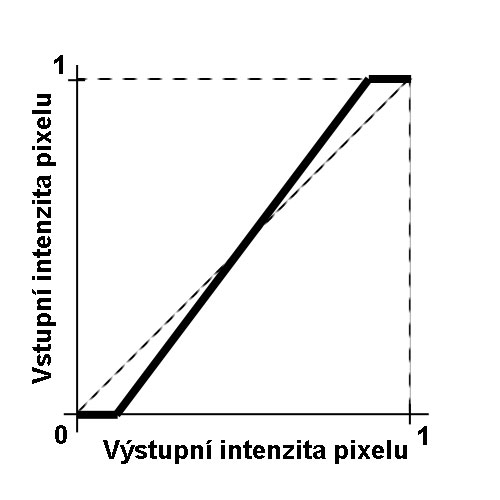
\includegraphics[width=0.4\textwidth,height=0.4\textwidth]{Text/IMG/Kontrast_Transformace_1.jpg}
		&
			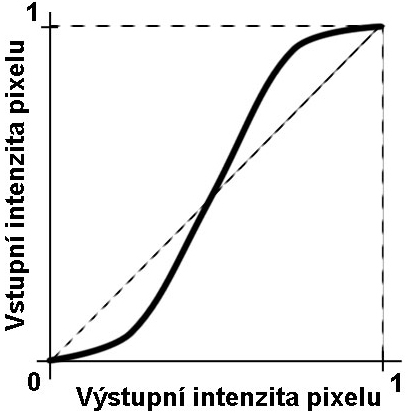
\includegraphics[width=0.4\textwidth,height=0.4\textwidth]{Text/IMG/Kontrast_Transformace_2.jpg}
		\end{tabular}
	\caption{Změna kontrastu pomocí lineární (vlevo) a nelineární (vpravo) transformace. V prvním případě dochází a ve druhém nedochází ke ztrátě informace.}
\end{table}



\subsection{Kontrast nelineárním způsobem}
S využitím jazyka Cg (případně C++ při odstranění OpenGL) lze implementovat nelineární změnu kontrastu zachovávající všechny informace v obrázku. V následující stati najdeme jednu z možných funkcí pro tuto transformaci.

Cílem je najít matematickou funkci, jež se svým grafem blíží grafu v tabulce \ref{kontrast} vrpavo. Podobný průběh má funkce $tanh(c\cdot x)$ na intervalu $(-\infty,\infty)$, kde parametr $c$ určuje derivaci v bodě $0$.

Graf funkce posuneme do bodu  $[\frac{1}{2},\frac{1}{2}]$:

\begin{equation}
f(x) = tanh(c\cdot(x-\frac{1}{2})) + \frac{1}{2}
\end{equation}

Omezíme obor hodnot na interval: $[0,1]$:

\begin{equation} \label{tanh1}
f(x) = \frac{1}{2}\cdot tanh(2\cdot c\cdot(x-\frac{1}{2})) + \frac{1}{2}
\end{equation}

Graf funkce \ref{tanh1} neprochází body $[0,0]$, $[1,1]$. Proto přičteme k funkci jednoduchou lineární funkci:

\begin{equation}
f(x) = k\cdot(x-\frac{1}{2}) + \frac{1}{2}\cdot tanh(2\cdot c\cdot(x-\frac{1}{2})) + \frac{1}{2}
\end{equation}

Lze odvodit, že ke splnění podmínek: $f(0)=0$ a $f(1)=1$ je třeba aby:

\begin{equation}
k = 1 - tanh(c)
\end{equation}

Dosazením dostáváme výsledný tvar funkce:

\begin{center}
\framebox{ $f(x) = (1 - tanh(c))\cdot(x-\frac{1}{2}) + \frac{1}{2}\cdot tanh(2 \cdot c\cdot(x-\frac{1}{2})) + \frac{1}{2} $ }
\end{center}

V tabulce \ref{kontrast} vidíme graf pro c=1 a c=2.


\noindent
\begin{table}[ht]
	\label{kontrast}
	\centering
		\begin{tabular}{p{0.3\textwidth}p{0.3\textwidth}}
			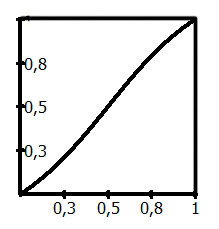
\includegraphics[width=0.3\textwidth,height=0.3\textwidth]{Text/IMG/nelinearni1.jpg}
		&
			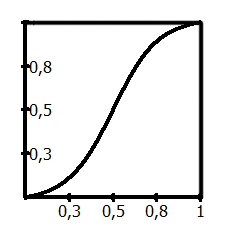
\includegraphics[width=0.3\textwidth,height=0.3\textwidth]{Text/IMG/nelinearni2.jpg}
		\end{tabular}
	\caption{Graf nalezené funkce pro nelineární změnu kontrastu pro $c=1$ (vlevo) a $c=2$ (vpravo).}
\end{table}


\newpage
\subsection{Kontrast a světlost v OpenGL}
Pro realizaci jednoduchých barevných transformací snímku disponuje knihovna OpenGL funkcemi Bias a Scale.

\begin{itemize}
\item Voláním funkce Bias s parametry K,B provedeme přičtení konstanty K k hodnotě barevné složky B pro všechny pixely obrázku.
\item Voláním funkce Scale s parametry K,B provedeme vynásobení stávající barevné složky B konstantou K pro všechny pixely obrázku.
\end{itemize}

Transformační křivky obou funkcí vidíme v tabulce \ref{biasscale}. Funkce Bias odpovídá změně jasu snímku. Změnu kontrastu musíme realizovat pomocí volání obou funkcí se správně dopočítanými parametry.

Pro změnu kontrastu voláme nejdřív funkci Scale s parametrem $s$, pak funkci Bias s parametrem $b$. Výsledek odpovídá transformaci:
 
\framebox{ $ y = s \cdot x + b$ }

Vztah mezi parametry $b$ a $s$ takový, aby transformační křivka procházela bodem [0.5,0.5], je:

\framebox{ $b=\frac{1}{2}\cdot(1-s)$ }

\noindent
\begin{table}[ht]
	\label{biasscale}
	\centering
		\begin{tabular}{p{0.35\textwidth}p{0.35\textwidth}}
			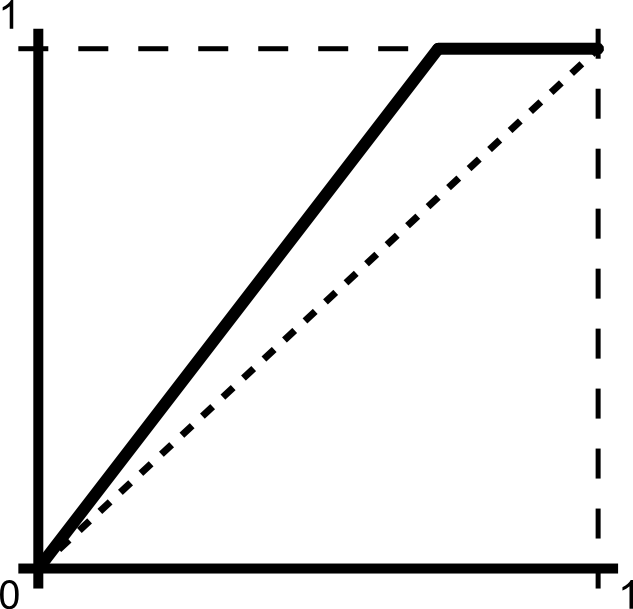
\includegraphics[width=0.3\textwidth]{Text/IMG/Bias.png}
		&
			\includegraphics[width=0.3\textwidth]{Text/IMG/Scale.png}
		\end{tabular}
	\caption{Křivka transformací Bias (vlevo) a Scale (vpravo). Jejich správnou kombinací lze dosáhnout změny kontrastu.}
\end{table}

<< neskudla >>




\begin{comment}
\subsection{Kontrast v knihovně Cg toolkit}
Knihovna Cg toolkit nabízí oproti OpenGL programování výpočtů s barevnými složkami. Pomocí funkce tex2D si zjistíme barevné složky původního pixelu, s nimi pak můžeme provádět libovolné operace a výsledek pak uložit do výstupu.
\subsection{Kontrast lineární transformací}
Knihovna Cg opět nedisponuje funkcí pro změnu kontrastu, ale podobně jako v předchozím případě si můžeme změnu kontrastu naprogramovat sami - v tomto případě mnohem přehlednějším způsobem. Násobme barevné hodnoty pixelu koeficientem a přičtěme adekvátní konstantu. To v Cg zapíšeme takto:
\begin{lstlisting}[label=DicomImageClass,caption={...}]
C3E3f_Output main(float2 texCoord : TEXCOORD0, uniform sampler2D decal : TEX0, uniform float brightness){
  C3E3f_Output OUT;
  OUT.color = tex2D(decal,texCoord)*scale + bias;
  return OUT;
}
\end{lstlisting}
Ve srovnání s OpenGL je tato implementace výrazně přehlednější. Podíváme-li se na řádek 3, vidíme hned zápis transformační funkce ve tvaru: f(x) = k*x - z. 
Změna jasu pak bude provedena přičtením konstanty bez násobení: \clist{OUT.color = tex2D(decal,texCoord)*scale}.
\end{comment}





\section{Rychlost vykreslování}
Jednou z otázek na kterou se snaží najít odpověď tento VÚ je to, zda by bylo možné z programu odstranit knihovny OpenGL a Cg toolkit. Jedná se o knihovny zajišťující práci s grafickými daty, hlavně se pak jedná o knihovnu výrazně urychlující zobrazování grafických dat. Před odstraněním knihoven z programu musíme nejprve zjistit, zda bude možné realizovat zobrazování dodstatečně rychle i bez těchto knihoven. 

Při vývoji DicomPresenteru byl kladen důraz na dostatečně plynulé ovládání. Pro práci s jakoukoliv aplikací je pohodlné, je-li mezi uživatelskou akcí a její realizací co nejkratší prodleva. V DicomPresenteru jsou výpočetně nejnáročnejčí akce: přesouvání snímků po obrazovce, úprava jasu a kontrastu snímků. Průměrný počet vykreslených snímků za sekundu při těchto akcích je při využití OpenGL 90 fps. Odhad toho, jak rychle poběží program bez OpenGL a Cg toolkit můžeme udělat tak, že naprogramujeme dvě aplikace, které budou mít na starosti pouze dvě zmiňované akce (posun snímku, změnu kontrastu). Jeden program bude využívat knihovny, druhý ne. Výkon testovacích aplikací a DicomPresenteru se bude jistě značně lišit\footnote{Rozdíl v rychlosti vykreslování u DicomPresenteru a testovacích aplikací je způsoben tím, že DicomPresenter vedle vykreslování dat na obrazovku musí řešit další úlohy: zachytávání uživatelských akcí, předávání uživatelských akcí napříč objektovým modelem, vykreslování ovladacích prvků, vykreslování textů.}, ale z naměřených hodnot lze odhadnout, jak rychle poběží DicomPresenter bez OpenGL a Cg toolkit. Uvažujme nyní pouze jednu z úloh: označme si $fps_{lib}$ počet naměřených snímků za sekundu v aplikaci využívající knihovny, $fps_{software}$ počet naměřených fps v aplikaci nevyužívající grafické knihovny, $fps_{dp}$ nechť je průměrný počet snímků kterého dosahuje DicomPresenter. Pak spodní odhad\footnote{Vykreslování na obrazovku je jen část úloh, které DicomPresenter řeší v každém kroku. Zpomalíme-li tuto část n-krát, bude pak běh programu v nejhorším případě n-krát pomalejší.} průměrného počtu snímků, kterého bude dosahovat DicomPresenter bez OpenGL a Cg toolkit v dané úloze je:

\begin{equation}
fps_{odhad} = \frac{fps_{software}}{fps_{lib}} \cdot fps_{dp}
\end{equation}

\subsection{Změna kontrastu bez Cg toolkit}

\begin{lstlisting}[label=DicomImageClass,caption={...}]
for (int y = 0; y<h; y++){
	Rgb = (QRgb*)ShowImage.scanLine(y);
	for ( int x = 0; x < w; x++ ){
		Rgb[x] = qRgb(qRed(Rgb[x])*c+0.5*(1-c),qGreen(Rgb[x])*c+0.5*(1-c),qBlue(Rgb[x])*c+0.5*(1-c));
	}
}
\end{lstlisting}

\subsection{Změna kontrastu v Cg toolkit}

\begin{lstlisting}[label=DicomImageClass,caption={...}]
C3E3f_Output main(float2 texCoord :TEXCOORD0, uniform sampler2D decal :TEX0, uniform float contrast){
  C3E3f_Output OUT;
  OUT.color = tex2D(decal,texCoord)*contrast+0.5(1-contrast);
  return OUT;
}
\end{lstlisting}

\subsection{Posun snímku bez OpenGL}
\begin{lstlisting}
void Workspace::draw(QPoint leftTop, QImage *sourceImage){
	int width = sourceImage->width();
	int height = sourceImage->height();
	int xPos = leftTop.x();
	int yPos = leftTop.y();
	for ( int y = 0; y < this->height(); y++ ){
		QRgb *workspaceImageLinePtr = (QRgb*)this->scanLine(y);
		for ( int x = 0; x < this->width(); x++ ){
			workspaceImageLinePtr[x] = qRgb(0,0,0);
		}
	}
	for ( int y = 0; y < height; y++ ){
		QRgb *sourceImageLinePtr = (QRgb*)sourceImage->scanLine(y);
		QRgb *workspaceImageLinePtr = (QRgb*)this->scanLine(yPos + y);
		for ( int x = 0; x < width; x++ ){
			workspaceImageLinePtr[xPos + x] = qRgb(qRed(sourceImageLinePtr[x]),qGreen(sourceImageLinePtr[x]),qBlue(sourceImageLinePtr[x]));
		}
	}
}
\end{lstlisting}

\subsection{Posun snímku s OpenGL}

\begin{lstlisting}
void GLPainter::Paint(int translationX){
	glClear(GL_COLOR_BUFFER_BIT);
	float ratio = (float)translationX/im->width().;
	glBegin(GL_POLYGON);
		glColor3f (Brightness, Brightness, Brightness);
		glTexCoord3f(0.0,0.0,0.0);	glVertex3f(ratio+ -1.0, -1.0, 0.0 );
		glTexCoord3f(0.0,1.0,0.0);	glVertex3f(ratio+ -1.0,  1.0, 0.0 );
		glTexCoord3f(1.0,1.0,0.0);	glVertex3f(ratio+  0.0,  1.0, 0.0 );
		glTexCoord3f(1.0,0.0,0.0);	glVertex3f(ratio+  0.0, -1.0, 0.0 );
	glEnd();
}
\end{lstlisting}






























\begin{comment}

\subsection{Implementace v Qt}
Grafická část rozhraní knihovny Qt je dělaná čistě pro dvojrozměrnou grafiku a všechny výpočty jsou prováděny jen na procesoru. Chceme-li měnit světlost snímku, musíme procházet for-cyklem všechny body obrázku a provést operaci pro každý bod zvlášť. Pokud navíc zadáme světlost pixelu mimo požadovanou mez, program se zasekne. Narozdíl od toho knihovny OpenGL i Cg automaticky barevnou hodnotu pixelu oříznou na přípustnou mez.

Intuitivní, avšak pomalejší implementace v Qt knihovně vypadá následovně:

\begin{lstlisting}[label=DicomImageClass,caption={...}]
for (int y=0; y<h; y++){
	for (int x=0; x<w; x++){
		Rgb = MemoryImage.pixel(x,y);
		Rgb = qRgb(qRed(Rgb)*cont,qGreen(Rgb)*cont,qBlue(Rgb)*cont);
		ShowImage.setPixel(x,y,Rgb);
	}
}
\end{lstlisting}

V úryvku kódu vidíme zejména procházení celého obrázku ve dvou for-cyklech(řádky 13,14). V každém kroku si zjistíme barevné souřadnice pixelu, upravíme je a uložíme je. To má na starosti procesor a jedná se o největší handicap celého programu. Při této implementaci je úloha zpracována sériově na jednom jádře, jak je vidět z následujících grafů sledujících zátěž jednotlivých jader:

\hspace{1cm}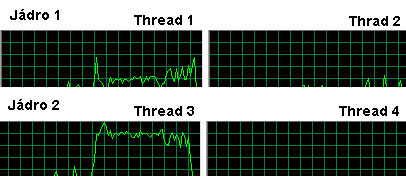
\includegraphics[width=0.8\textwidth]{Text/IMG/MultiThread.jpg}

Procesor je fyzicky dvoujádrový, ale operační systém jej vidí jako čyřjádrový. Celý výpočet probíhal viditelně v třetím threadu, v prvním pak běžely zřejmě jen pomocné operace, další 2 thready zůstaly nevyužité.

Chceme-li výpočet urychlit, můžeme tak udělat v několika krocích:

Nebudeme si ukládat barevné souřadnice původního obrázku do proměnné, tam je upravovat a ukládat zpět na půbodní místo. Ale necháme si předat ukazatel na místo v paměti, kde je obrázek uložen, a výsledek ukládat přímo tam.

Dále nebudeme volat funkci, která nám na základě souřadnic vrátí barevné složky obrázku, ale necháme si od Qt knihovny předat ukazatel na celý jeden řádek obrázku. Tím se vyhneme opakovanému volání funkce.

Dvojice for-cyklů procházející obrázek bude nahrazena tímto kódem:

\begin{lstlisting}[label=DicomImageClass,caption={...}]
for (int y = 0; y<h; y++){
	Rgb = (QRgb*)ShowImage.scanLine(y);
	for ( int x = 0; x < w; x++ ){
		Rgb[x] = qRgb(qRed(Rgb[x])*cont,qGreen(Rgb[x])*cont,qBlue(Rgb[x])*cont);
	}
}
\end{lstlisting}

Jak je vidět, v každém řádku obrázku ušetříme hned dvě volání funkce pro každý pixel. Zkusme si spočítat kolik funkčních volání jsme ušetřili:

V prvním případě voláme pro každý pixel funkce QImage::pixel() a QImage::setPixel(). Rozměr obrázku je 512*512 pixelů. To jest: 512*512*2 = cca 500 000 funkčních volání.

V druhém případě voláme pouze funkci QImage::scanLine pro každý řádek obrázku, tj. 512*2 = 1024 volání.

Jak je vidět, jedná se o zredukování počtu volání nějaké funkce o dva řády. Výsledek takového zjednodušení uvidíme v závěru kapitoly.


\subsection{Implementace v OpenGL}

OpenGL je knihovna přímo určená pro urychlení grafických výpočtů a jejich zjednodušenou obsluhu. Hlavní rozdíl oproti implementaci v Qt je ten, že výpočty neprobíhají na procesoru, ale na grafické kartě, což je, jak se později ukáže, zásadní rozdíl ve výkonnosti programu. Stejně tak data nejsou uložena v modulech paměti RAM na základní desce, ale jsou v paměti grafické karty.

Implementace vypadá následovně:

\begin{lstlisting}[label=DicomImageClass,caption={...}]
start = time (NULL);
for (int j=0; j<10; j++){
	float Brightness=0.0;
	for (int i=0; i<1000; i++){
		Brightness = Brightness+0.001;
		gl->Paint(Brightness);
		w.updateGL();
	}
}
end = time (NULL);

void GLPainter::PrepareTexture() {
	glBindTexture( GL_TEXTURE_2D, TextureIdentifier );
	gluBuild2DMipmaps( GL_TEXTURE_2D, 3, width, height, GL_RGB, GL_UNSIGNED_BYTE, TextureData );
	glEnable( GL_TEXTURE_2D );
}

void GLPainter::Paint(float Brightness){
	glBegin(GL_POLYGON);
		glColor3f (Brightness, Brightness, Brightness);
		glTexCoord3f(0.0,0.0,0.0);	glVertex3f( -1.0, -1.0, 0.0 );
		glTexCoord3f(0.0,1.0,0.0);	glVertex3f( -1.0,  1.0, 0.0 );
		glTexCoord3f(1.0,1.0,0.0);	glVertex3f(  1.0,  1.0, 0.0 );
		glTexCoord3f(1.0,0.0,0.0);	glVertex3f(  1.0, -1.0, 0.0 );
	glEnd();
}
\end{lstlisting}
Na první pohled lze vidět nesrovnatelné zjednodušení kódu, zatímco v prvním případě (Qt) jsme museli procházet celý obrázek po pixelech, zde můžeme využít funkce knihovny OpenGL pomocí které lze měnit světlost jejího výstupu.

V programu si nejprve snímek uložíme do paměti jakožto OpenGL texturu (řádky 12-16), posléze provádíme vykreslování této textury na načrtnutý obdélník (18-26).


\subsection{Iplementace v Cg}

Knihovna Cg slouží k programování výpočtů na čipu grafické karty. V jednoduchém jazyku podobném jazyku C popíšeme prováděné výpočty pro změnu světlosti. Výpočty jsou pak realizovány na speciálním hardwarovém čipu (pixel shader, vertex shader). Přínos pixel a vertex shaderů je v nové paletě efektů, jež je možno provádět, a dále ve výrazném urychlení těchto efektů.

Podívejme se na implementaci programu s využitím Cg, tentokráte výpočty nebyly prováděny jen v prostředí jazyka C++, ale i v jazyce Cg.

\begin{lstlisting}[label=DicomImageClass,caption={...}]
start = time (NULL);
for (int j=0; j<10; j++){
	float Brightness=0.0;
	for (int i=0; i<1000; i++){
		Brightness = Brightness+0.001;
		gl->Paint(Brightness);
		w.updateGL();
	}
}
end = time (NULL);

void GLPainter::PrepareTexture() {
	glBindTexture( GL_TEXTURE_2D, TextureIdentifier );
	gluBuild2DMipmaps( GL_TEXTURE_2D, 3, width, height, GL_RGB, GL_UNSIGNED_BYTE, TextureData );
	glEnable( GL_TEXTURE_2D );
}

void GLPainter::changeBrightness( float Brightness ){
	cgGLBindProgram(Program);
	cgGLEnableProfile(Profile);
	cgSetParameter1f(hBright, Brightness);
	cgUpdateProgramParameters (Program);
	cgGLDisableProfile(Profile);

	Paint();
}

void GLPainter::Paint(){
	glClear(GL_COLOR_BUFFER_BIT);

	cgGLBindProgram(Program);
	cgGLEnableProfile(Profile);
	cgGLEnableTextureParameter(hDecal);

	glBegin(GL_POLYGON);
		glTexCoord3f(0.0,0.0,0.0);	glVertex3f(-1.0,-1.0,0.0);
		glTexCoord3f(0.0,1.0,0.0);	glVertex3f(-1.0,1.0,0.0);
		glTexCoord3f(1.0,1.0,0.0);	glVertex3f(1.0,1.0,0.0);
		glTexCoord3f(1.0,0.0,0.0);	glVertex3f(1.0,-1.0,0.0);
	glEnd();

	cgGLDisableProfile(Profile);
	cgGLDisableTextureParameter(hDecal);
}
\end{lstlisting}

\begin{lstlisting}[label=DicomImageClass,caption={...}]
struct C3E3f_Output {
  float4 color : COLOR;
};

C3E3f_Output main(float2 texCoord : TEXCOORD0, uniform sampler2D decal : TEX0, uniform float brightness)
{
  C3E3f_Output OUT;
  OUT.color = tex2D(decal,texCoord)*brightness;

  return OUT;
}
\end{lstlisting}

První část programu je shodná s předchozí verzí (opět je volána knihovna OpenGL). Rozdíl však začíná od řádku 18. Ve funkci changeBrightness() musíme volat funkce knihovny Cg toolkit pomocí kterých předáme pixel shaderu parametr určující změnu světlosti. Před samotným vykreslováním pomocí OpenGL (řádky 35-40) musíme nechat program zkompilovat na čipu grafické karty a nastavit, aby ovlivňoval výstup OpenGL.

Za povšimnutí stojí fakt, že výpočet změny světlosti se přesunul z kódu C++ do Cg. Změna světlosti je popsána v samostatném programu jež se kompiluje na grafické kartě.


\subsection{Porovnání výpočtů}

Popsané programy byly testovány na počítačové sestavě:

Intel Core i3, ATI Radeon 5470. Takt procesoru je 2,26 GHz

Jedná se o dvoujádrový procesor, pro výpočet však bylo použito pouze jedno jádro. Takt GPU na grafické kartě je 750MHz.

V každé konfiguraci jsme požadovali jiný počet cyklů programu, jenom z důvodu časové úspory při ladění.

\begin{tabular}{| p{5cm} | l | l | l | }
  \hline                       
  Typ konfigurace & Počet cyklů & Čas & Snímků za vteřinu \\
  \hline
  \hline
  Qt (bez přímého přístupu do paměti)& 100 & 4 sekundy & 25 fps\\
  \hline
  Qt (s přímým přístupem do paměti)& 1000 & 11 sekund & 90 fps\\
  \hline
  Qt, OpenGL & 10 000 & 16 sekund & cca 600  fps \\
  \hline
  Qt, OpenGL, Cg & 10 000 & 14 sekund & cca 700 fps \\
  \hline  
\end{tabular}

Jak je vidět z naměřených údajů, s použitím knihovny OpenGL se dá dosáhnout úctihodného výkonu při vykreslování snímků v programu. Nicméně vezmeme-li v úvahu fakt, že standardní rychlost snímání ovládacích zařízení přes USB v operačním systému je 125Hz a dále obnovovací frekvence u monitoru nebývá zpravidla vyšší než 100Hz, musíme uznat, že výkon dosažený pomocí OpenGL je nadbytečný. To by určitě nevadilo a velká rezerva ve výkonu by mohla být zárukou plynulého chodu programu i za ztížených podmínek (uživatel využívá procesor i jiným způsobem za běhu programu), ale bohužel přítomnost knihovny OpenGL v programu má za důsledek značné problémy s provozem programu na méně výkonných, či starších grafických kartách. Byly zjištěny problémy s provozem programu na integrovaných grafických kartách Intel, které však jsou velice často instalovány do moderních notebooků.

Výkon programu, při pomalejší implementaci v Qt knihovně, kdy jsme nevyužívali manuálního přístupu do paměti, ale k tomuto jsme používali implementované funkce v Qt knohovně, je spíše nedostačující. Dosažený výkon v testovacím programu: 25 snímků za vteřinu sice sám o sobě dostačující je, ale musíme vzít v úvahu ten fakt, že se jednalo o velice primitivní testovací program, který nedělal nic jiného než přepočet barevných složek obrázku a jeho zobrazení. DicomPresenter vedle toho musí vykreslovat ovládací prvky programu, což znamená několik funkčních volání navíc.

Oproti tomu výkon dosažený pomocí pokročilé implementace, kdy přistupujeme ručně do paměti počítače a obrazová data měníme tam, by měl být dostačující pro běh reálného programu. I při výrazném zpomalení aplikace kvůli přepočítávání zobrazovaných ovládacích prvků, bychom se měli bezpečně udržet nad hranicí 30FPS.

Závěrem této kapitoly je nutno podotknout, že Knihovny OpenGL, Cg z programu odstranit lze a v nejbližší době bude takto učiněno. Program by se tak měl stát výrazně bezproblémovější, co se týče provozu v praxi. Měl by být kompatibilní s převážnou většinou počítačových sestav - to je však nutná podmínka pro to, aby program mohl být v praxi použitelný.


\end{comment}

\section{}

\newpage
\chapter{DCMTK}
\section{Problém s načítáním DICOM snímků}
Situace na poli prohlížečů lékařských snímků je dosti komplikovaná. V práci\cite{flaska} na str. 10 je to blíže vysvětleno: Prohlížeče DICOM snímků jsou buď komerčními placenými produkty a nebo jsou volně šiřitelné, ale nedosahují takových kvalit. Při vývoji DicomPresenteru byl program testován na určité množině snímků (např. archiv ženevské university\citesec{DicomSamples}). Velice známý prohlížeč Medinria, pak nezanedbatelnou část těchto snímků nedokázal správně zobrazit (buď je nenačetl vůbec, nebo je zobrazil s chybami). Tento fakt jen dokazuje to, že volně šiřitelné prohlížeče jsou zatím zpravidla ve fázi vývoje a vývoj DicomPresenteru tak má smysl, neboť pomyslný trh zatím není žádným významným prohlížečem obsazen (jiná situace je u Mac OS X\footnote{Pro operační systém Mac OS X byl vytrořen velice úspešný prohlíčeč OsiriX. Z tohoto důvodu není moc vhodné DicomPresenter v budoucno portovat pro Mac OS X, neboť tam má prohlížeč silnou konkurenci a tak by o něj zřejmě málokdo jevil zájem.}).

S podobnými problémy s jakými se potýkají volně šiřitelné prohlížeče se však potýká i DicomPresenter. Při rozsáhlejším testování programu na větší množině dat nastal problém, že prohlížeč nedokázal načíst poměrně rozsáhlou skupinu DicomSnímků (jiná část snímků ze zmíněného archivu), navíc prohlížeč při pokusu o načtení takového snímku zhavaroval. To se jevilo jako dost závažný problém.

Při bližším zkoumání, proč snímky nelze nalézt, se podařilo objevit, v které části kódu nastává problém:

\begin{lstlisting}[label=DicomImageClass,caption={Při otevírání snímku aplikace havarovala, k pádu aplikace došlo ve funkci \clist{CDicomFramed::LoadDicomImage} na uvedeném řádku (zde řádek 3).}]
bool CDicomFrames::LoadDicomImage(char *fileName, bool isFirst, int framesCount ) {
 	...
	iDicomImage = new DicomImage (fileName);
	...	
}
\end{lstlisting}

Konstruktor třídy \clist{DicomImage} je definovám v knihovně DCMTK.

\begin{lstlisting}[label={DicomImage},caption={Definice konstruktoru třídy \clist{DicomImage}.}]
DicomImage::DicomImage (const char *filename,
    const unsigned long flags = 0,
    const unsigned long fstart = 0,
    const unsigned long fcount = 0)
{
...
}
\end{lstlisting}

Hodnota předávané proměnné ukazatelem \clist{fileName} byla: \clist{"C:/Dev/Samples/IMG-0001-0001.dcm"}.

V uvedené části kódu není možné nalézt chybu, kterou by programátor udělal. Problém tedy vznikal někde uvnitř knihovny \clist{dcmtk}, která nedokázala správně načíst požadovaný soubor. Zdůrazněme ještě, že se jednalo o DICOM soubory z archivu Ženevské universitní nemocnice určené pro studijní účely.

\subsection{Hledání příčiny selhání}
Jak bylo popsáno výše, knihovna DCMTK zhavarovala při načítání DICOM snímku, nebylo však možné zjistit, v které části dcmtk knihovny nastal problém. Pro bližší diagnostiku problému v externí knihovně je potřeba si knihovnu přeložit v debug verzi, kdy si pak můžeme nechat vypsat konkrétní řádek na kterém nastala chyba (viz. str. \pageref{releasedebug}).
Po přeložení aplikace v Debug verzi program po načtení stejného snímku nezhavaroval, jen na obrazovce nebylo nic vidět. Díky tomu, že program nezhavaroval můžeme si pomocí diagnostické funkce DCMTK knihovny nechat vypsat informace o tom, jak načítání snímků dopadlo. Použití takových diagnostických funkcí je běžná praxe u knihoven. Uveďme několik příkladů diagnostických funkcí u  n některých knihoven:

\hspace{-1cm}
\begin{tabular}{| p{3cm} | p{3cm} | p{2cm} | p{6cm} | }
  \hline                       
  Knihovna & Funkce & Typ & Příklady \\
  \hline
  \hline                     
  OpenGL & glGetError() & GLenum & GL\_INVALID\_VALUE, GL\_OUT\_OF\_MEMORY\\
  \hline
  Cg toolkit & cgGetError()  & CGerror & CG\_NO\_ERROR, CG\_COMPILER\_ERROR\\
  \hline
  .NET4 System\-.Windows\-.Forms & GetError(Control) & String & System\-::Argument\-Exception, System::IO\-::Directory\-NotFound\-Exception\\
  \hline
\end{tabular}

Knihovna DCMTK nám umožňuje pomocí diagnostické funkce \clist{DicomImage::getStatus()} zjistit stav v jakém se objekt nachází, tzn. můžeme zjistit, jak dopadlo načítání snímku.

\begin{lstlisting}[label={xxx}]
iDicomImage = new DicomImage (fileName);

EI_Status imageStatus;
imageStatus = iDicomImage->getStatus();
\end{lstlisting}

\clist{EI\_Status} je výčtový typ, tzn. proměnná typu \clist{EI\_Status} může nabývat omezené množiny hodnot (např. EIS\_Normal, EIS\_InvalidValue).

Pomocí funkce \clist{DicomImage::getStatus()} bylo tedy možné zjistit, že v debug verzi načítání snímku proběhně s chybou, a to konkrétně:

 \clist{EIS\_MissingAttribute}

Po zkoumání, co tato chyba znamená, vyplynulo, že načítaný DICOM soubor nemá svou hlavičku v odpovídajícím formátu. Lze se dohledat, že nástroj: \clist{gdcmconv} dokáže nevyhovující hlavičku DICOM souboru převést do univerzálního tvaru, který bude akceptovat i knihovna DCMTK.

\subsection{Integrace externího nástroje do programu}
Zmiňovaný nástroj \clist{gdcmconv} dokáže opravit nekompatibilní hlavičku DICOM souboru. Otázkou bylo, jak tento nástroj do našeho programu integrovat. Nabízely se dvě odlišné varianty. První variantou by bylo:

\begin{itemize}
\item
Přeložit zdrojový kód programu \clist{gdcmconv} tak, že si vytvoříme C++ knihovnu. Knihovnu pak připojíme do programu DicomPresenter tak, že funkce programu \clist{gdcmconv} budeme moct používat uvnitř našeho programu.
\end{itemize}

Problém však je v tom, že program DicomPresenter už tak závisí na šesti různých knihovnách a tím se značně komplikuje jeho překlad. Při překladu aplikace by se pak programátor musel vázat na další knihovnu a musel by vždy obstarat zdrojový kód knihovny a přeložit si ji do \clist{.lib} souborů. V případě, že by zdrojový kód nenašel, nebo by se mu knihovnu programu \clist{gdcmconv} nepodařilo přeložit, nemohl by pak přeložit ani program DicomPresenter. Více o problematice překladu programu závislého na několika externích knihovnách v části \ref{sec:preklad} (str. \pageref{sec:preklad}). Proto tedy druhá varianta:

\begin{itemize}
\item
Obstarat program \clist{gdcmconv} jakožto spustitelný soubor. \clist{gdcmconv} pak spouštět v C++ jako externí program funkcí \clist{system(...)}.
\end{itemize}

Tato možnost se jevila jako vhodnější. Pro překlad DicomPresenteru nebude potřeba zdrojový kód programu \clist{gdcmconv}, bude stačit hotový program zkopírovat do adresáře DicomPresenteru. Pokud programátor nebude schopný program obstarat, DicomPresenter poběží i bez něj za cenu, že nebude možné otevřít určité DICOM soubory.

Po těchto úvahách byla implementována druhá možnost řešení. Kód funkce \clist{LoadDicomImage} (viz. kód \ref{DicomImageClass}) byl upraven následujícím způsobem:

\begin{lstlisting}[label={xxx}]
bool CDicomFrames::LoadDicomImage(char *fileName, bool isFirst, int framesCount ) {
	iDicomImage = new DicomImage (fileName);
	EI_Status imageStatus = iDicomImage->getStatus();

	if (imageStatus==EIS_MissingAttribute){			
		QString strCommand("gdcmconv --raw --force ");
		strCommand.append(fileName);
		strCommand.append(" temp.dcm");
		int i = system(strCommand.toAscii().data());
		if(i==0){
			iDicomImage=NULL;
			iDicomImage = new DicomImage ("temp.dcm");
			remove("temp.dcm");
		}else{
			QMessageBox msgBox;
			msgBox.setText("DICOM file is missing some header attribute.");
			msgBox.exec();
		}		
	}
 ...
}
\end{lstlisting}

Na řádku 3 si zjistíme, jak dopadlo načítání souboru. Pokud došlo k chybě (řádek 5), pak spouštíme externí program \clist{gdcmconv} s danými parametry (na řádcích 6-9) je sestavován celý příkaz. Příkaz:

\clist{gdcmconv --raw --force <nazevsouboru> temp.dcm}

nechá převést nevyhovující DICOM soubor na nový bezproblémový DICOM soubor. Pokud vytvoření nového souboru proběhně bez problému (řádek 10), pak je namísto původního souboru načten soubor nový. V opačném případě se uživateli objeví chybová hláška.

Po uvedené úpravě v kódu se výrazně zvýšil počet snímků, které DicomPresenter dokáže otevřít. Kód programu se nijak výrazně nezkomplikoval, ani by nový kus kódu neměl způsobit nějakou další chybu.




\newpage
\chapter{Multiplanární rekonstrukce}
Po předvedení programu v IKEM byl vznesen další požadavek na funkčnost programu a to implementace multiplanární rekonstrukce (MPR).

Multiplanární rekonstrukce je specifický způsob zobrazení snímku: Obrazovka je rozdělena na tři části. V každé části vidíme řez třírozměrného snímku a to ve třech na sebe kolmých rovinách. V každém z řezů dále vidíme vyznačené průsečíky se zbylými dvěma rovinami (viz Obrázek \ref{MPR}).

\begin{figure}
	\caption{Multiplanární rekonstrukce v programu \cite{volux}, na obrazovce je vidět snímek lidské lebky ve třech řezech (zepředu, z profilu, zespodu) a dále modelování objemu - to součástí DicomPresenteru nebude.}
	\begin{center}
	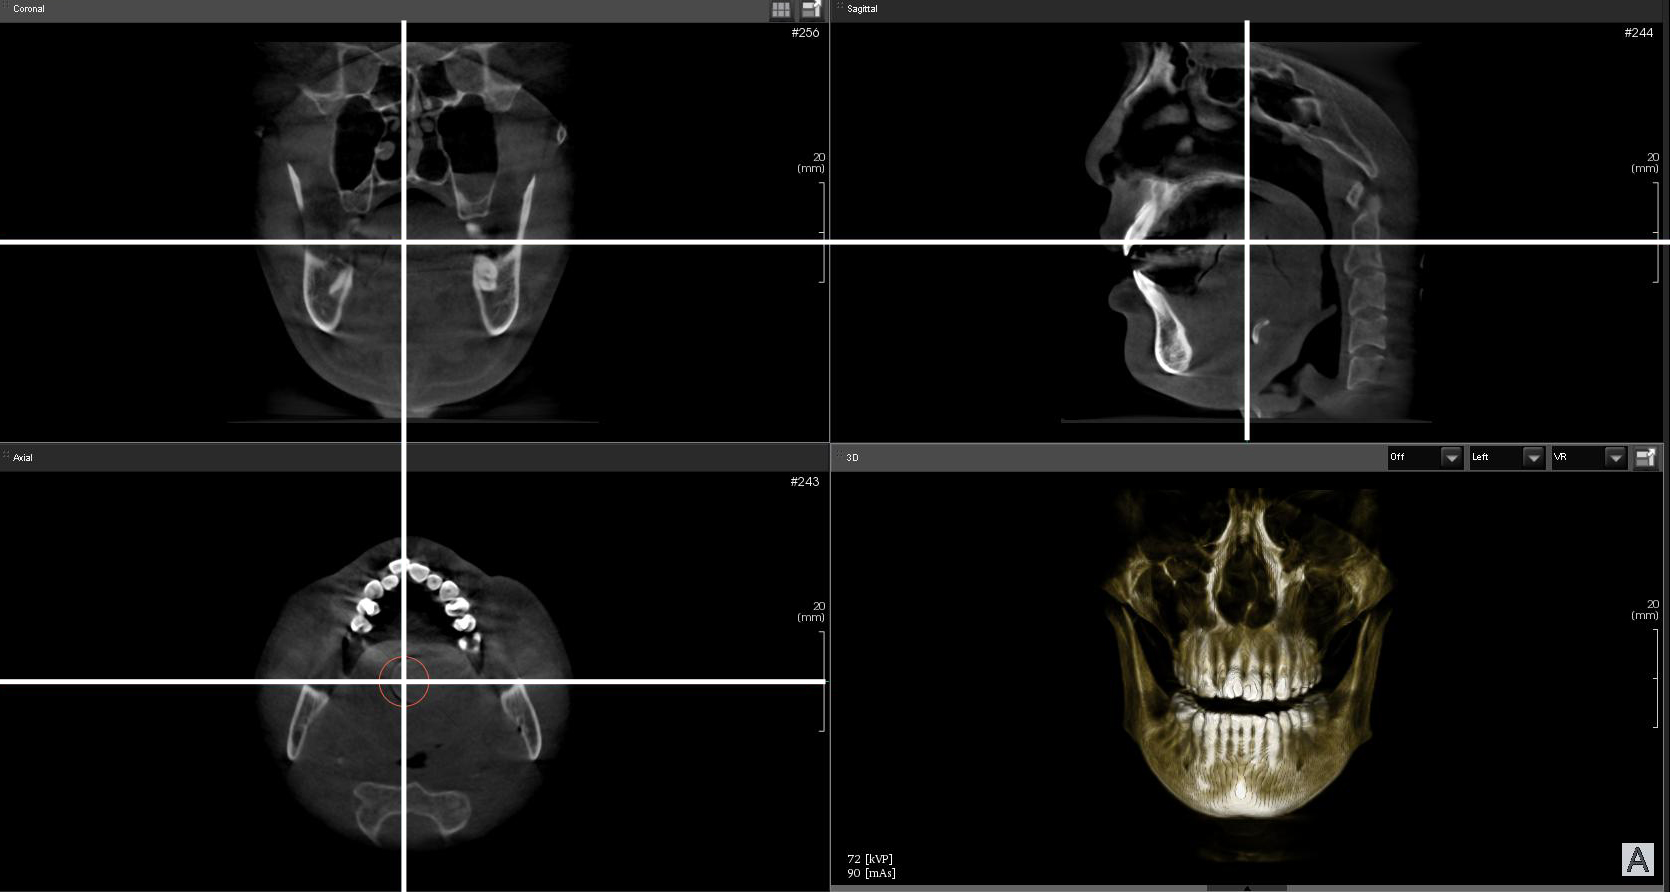
\includegraphics[width=0.7\textwidth]{Text/IMG/MPR.jpg}
	\end{center}
	\label{MPR}
\end{figure}

\section{Objektový návrh Dicom-Presenteru}
Zadání bylo do stávajícího programu přidat podporu multiplanární rekonstrukce. Jelikož přidání MPR znamená zásah do stávajícího objektového návrhu programu, je nutné se nejprve stručně seznámit se stávajícím objektovým návrhem programu.

V programu DicomPresenter je správa a vykreslování snímků řešeno použitím pěti základních tříd: Třída \clist{Image} reprezentuje snímek magnetické resonance. Třída \clist{Workspace} reprezentuje pracovní plochu na které máme otevřeno několik snímků typu \clist{Image}. Třída \clist{ImageExplorer} má na starost uložení snímků typu \clist{Image} v paměti počítače. Třídy \clist{WorkspaceExplorer} a \clist{WorkspaceManager} pak mají na starost přepínání mezi pracovními plochami a jejich uložení v paměti\footnote{Třídy \clist{Image}, \clist{Workspace}, \clist{ImageExplorer} mají na starost uložení dat v paměti i vykreslení dat na obrazovku a komunikaci s uživatelem. V případě správy pracovních ploch, kde je situace komplikovanější, jsou od sebe správa paměti a správa uživatelského rozhraní odděleny (třídy \clist{WorkspaceExplorer} a \clist{WorkspaceManager}). }. Náčrtek vztahů mezi třídami je na obrázku \ref{model}.

\begin{figure}
	\caption{Vztahy mezi objekty DicomPresenteru zajišťujícími správu pracovních ploch.}
	\begin{center}
		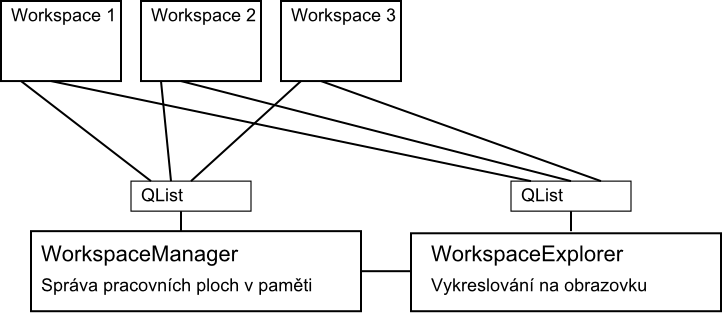
\includegraphics[width=0.7\textwidth]{Text/IMG/WorkspaceManager.png}
	\end{center}
	\label{model}
\end{figure}

Do tohoto modelu je nutné někam zařadit novou třídu, která zajistí funkčnost multiplanární rekonstrukce. Funkcemi multiplanární rekonstrukce nahrazuje to, co má na starosti třída Workspace. Otázkou bylo, zda vytvořit zcela novou třídu, nebo zda vložit nové funkce do stávající třídy Workspace, nebo zda rozdělit stávající třídu Workspace na dvě části a funkce společné pro oba typy pracovních ploch dědit. Po diskuzi byla vybrána první možnost a byla tak vytvořena třída nová, která nebude zobrazovat několik různých Dicom snímků, ale bude zobrazovat vždy jen jeden Dicom snímek v různých řezech. Bylo nutné zaručit, aby uživatel mohl přepínat mezi novou pracovní plochou s multiplanární rekonstrukcí a mezi všemi starými pracovními plochami.

\begin{comment}
\begin{figure}
	\caption{Vztahy mezi objekty DicomPresenteru zajišťujícími správu pracovních ploch.}
	\begin{center}
		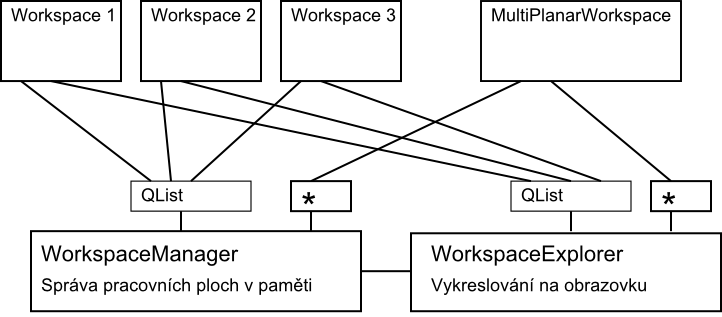
\includegraphics[width=0.7\textwidth]{Text/IMG/MultiPlanar.png}
	\end{center}
	\label{model}
\end{figure}
\end{comment}

\section{Implementace multiplanární rekonstrukce}
Multiplanární rekonstrukce byla naprogramována vytvořením nové třídy odpovídající pracovní ploše: PlanarWorkspace a dále úpravami v existující třídě Image.

\subsection{Třída PlanarWorkspace}
V třídě lze odlišit dvě části: funkce zpracovávající uživatelské akce, funkce zajišťující vykreslování výsledku na obrazovku.

Uživatelské akce jsou zachycovány funkcemi Qt knihovny \clist{QMouse\-Event\-::mouse\-Move\-Event()},\clist{QMouse\-Event\-::mouse\-Press\-Event()}. V odpovídajících funkcích z pozice kurzoru zjistíme s jakým řezem a jak má uživatel v úmyslu manipulovat\footnote{Uživatelské akce standardně zachycuje okno programu (třída Widget). Při stisku tlačítka myši třída Widget projde všechny základní prvky na obrazovce (\clist{Workspace}, \clist{WorkspaceExplorer} a \clist{WorkspaceManager}) a zjistí na který z nich uživatel klikl, všechny další akce pak směřuje tomuto prvku.}, to si uložíme do paměti počítače do proměnné \clist{planarCrossPosition}.

\begin{lstlisting}[label=DicomImageClass,caption={První část souboru \texttt{Window.cpp} se zdrojovým kódem třídy reprezentující okno programu.}]
void CGLPlanarWorkspace::mousePressEvent(QMouseEvent *event){
	if((event->x() < this->GetSize().x()/2)&&(event->y() < this->GetSize().y()/2)){
		UserManipulatingSlice = 'z';
		CGLWidget::GetInstance()->setCursor(QCursor(Qt::BlankCursor));
		iEventHistory->setX(event->x());	
		iEventHistory->setY(event->y());
		*iCursorHistory = QCursor::pos();
	}
  ...
}

void CGLPlanarWorkspace::mouseMoveEvent(QMouseEvent *event){
	QCursor::setPos(*iCursorHistory);
	if(UserManipulatingSlice == 'z'){
		int dx = event->x() - iEventHistory->x();
		int dy = iEventHistory->y() - event->y();
		if ((iPlanarCrossPosition.x+(float)dx/(float)iSensitivity>0.) && (iPlanarCrossPosition.x+(float)dx/(float)iSensitivity<1.))
			iPlanarCrossPosition.x=iPlanarCrossPosition.x+(float)dx/(float)iSensitivity;
		if ((iPlanarCrossPosition.y+(float)dy/(float)iSensitivity>0.) && (iPlanarCrossPosition.y+(float)dy/(float)iSensitivity<1.))
			iPlanarCrossPosition.y=iPlanarCrossPosition.y+(float)dy/(float)iSensitivity;
	}
	if(UserManipulatingSlice == 'x'){
 		...
	}
	if(UserManipulatingSlice == 'y'){
 		...
	}
	CGLWidget::GetInstance()->updateGL();
\end{lstlisting}

Vykreslování je řešeno ve funkci \clist{QGLWidget\-::Paint()}, to je třída Qt knihovny, kterou si předefinujeme podle potřeb. Ve funkci voláme nově definované funkce třídy \clist{Image}. Nejprve si vykreslíme tři požadované řezy do paměti grafické karty (frame buffer), pak kreslíme řezy na odpovídající místo na obrazovce. Souřadnice řezů jsou dopočítány podle proměnné \clist{planarCrossPosition}.

\begin{lstlisting}[label=DicomImageClass,caption={První část souboru \texttt{Window.cpp} se zdrojovým kódem třídy reprezentující okno programu.}]
void CGLImage::DrawToTextureSliceZ(TPlanarCrossPosition crossposition){
	glBindFramebufferEXT(GL_FRAMEBUFFER_EXT, iFBOZ);
	glBindTexture(GL_TEXTURE_3D, iTexture->GetTextureID());
	glBindTexture(GL_TEXTURE_2D, iSliceZ);
	glBegin(GL_QUADS);
	glColor4f(1.,0.,0.,1.);
	  glTexCoord3d(0,1,crossposition.z);  glVertex2d(0,0);
	  glTexCoord3d(1,1,crossposition.z);  glVertex2d(1,0);
	  glTexCoord3d(1,0,crossposition.z);  glVertex2d(1,1);
	  glTexCoord3d(0,0,crossposition.z);  glVertex2d(0,1);
	glEnd();
	glBindFramebufferEXT(GL_FRAMEBUFFER_EXT, 0);
}

void CGLImage::DrawSliceZ(){
	glBindTexture(GL_TEXTURE_2D, iSliceZ);
	glBegin(GL_QUADS);
	  glTexCoord2d(0,0);  glVertex2d(0,0.5);
	  glTexCoord2d(1,0);  glVertex2d(0.5,0.5);
	  glTexCoord2d(1,1);  glVertex2d(0.5,1);
	  glTexCoord2d(0,1);  glVertex2d(0,1);
	glEnd();
}
\end{lstlisting}








%%%%%%%%%%%%%%%%%%%%%%  DODATKY  %%%%%%%%%%%%%%%%%%%%%%

%\chapter{Dodatky}
%\section{Import kódu}
%\input{Text/07.Import.tex}

%%%%%%%%%%%%%%%%%%%%%%  LITERATURA  %%%%%%%%%%%%%%%%%%%%%%

\nocite{*}				% zobrazuj i necitovane primarni zdroje
\bibliography{Text/Literatura}
\nocitesec{*}				% sek. zdroje
\bibliographysec{Text/Zdroje}
\bibliographyurl{Text/Odkazy}


%%%%%%%%%%%%%%%%%%%%%%  PŘÍLOHY %%%%%%%%%%%%%%%%%%%%%%

% \chapter{Přílohy}

% \input{vnitrek_priloha1.tex} % pøíloha 1: vložená z externího souboru
% \input{vnitrek_priloha2.tex} % pøíloha 2: vložená z externího souboru



\end{document}

